\documentclass[aspectratio=169,11pt]{beamer}
\usepackage[utf8]{inputenc}
\usepackage[T1]{fontenc}
\usepackage[english]{babel}
\usetheme{Madrid}
\usecolortheme{whale}
\definecolor{uddblue}{HTML}{1F4E79}
\definecolor{uddlight}{HTML}{2E86C1}
\setbeamercolor{structure}{fg=uddblue}
\setbeamercolor{frametitle}{bg=uddblue,fg=white}
\setbeamercolor{title}{bg=uddblue,fg=white}
\setbeamercolor{block title}{bg=uddblue,fg=white}
\setbeamercolor{block body}{bg=uddblue!10}
\setbeamercolor{item}{fg=uddblue}
\usepackage{amsmath,amssymb}
\usepackage{graphicx}
\usepackage{booktabs}
\usepackage{listings}
\usepackage{tikz}
\usetikzlibrary{shapes,arrows,positioning,calc}
\lstset{language=R,basicstyle=\ttfamily\scriptsize,keywordstyle=\color{uddblue}\bfseries,commentstyle=\color{gray},stringstyle=\color{uddlight},backgroundcolor=\color{uddblue!5},frame=single,rulecolor=\color{uddblue!30},breaklines=true,showstringspaces=false}
\graphicspath{{figuras/}}
\titlegraphic{
\includegraphics[height=1.2cm]{logo_gobierno.png}}
\institute[CICS --- UDD]{Doctorado en Ciencias de la Complejidad Social --- CICS, UDD}
\newcommand{\highlight}[1]{\textcolor{uddlight}{\bfseries #1}}

\title[Regresi\'on Lineal M\'ultiple]{Regresi\'on Lineal M\'ultiple}
\subtitle{Sesi\'on 3 --- Econometr\'ia}
\author[A. Ag\"uero]{Amaru Ag\"uero}
\date{25 de marzo de 2026}

\begin{document}

% ============================================================================
% SLIDE 1: PORTADA
% ============================================================================
\begin{frame}
\titlepage
\end{frame}

% ============================================================================
% SLIDE 2: AGENDA
% ============================================================================
\begin{frame}{Agenda}
\begin{enumerate}
    \setlength{\itemsep}{3pt}
    \item De regresi\'on simple a m\'ultiple
    \item Sesgo de variable omitida (OVB)
    \item \textbf{Estructuras causales: confusora, collider, modificadora}
    \item \textbf{Modelos anidados e identificaci\'on de sesgos}
    \item Variables de control: cu\'ando y cu\'ales
    \item Variables categ\'oricas (dummy variables)
    \item T\'erminos de interacci\'on
    \item Pruebas de significancia (individual y conjunta)
    \item Multicolinealidad
    \item Implementaci\'on en R
\end{enumerate}
\end{frame}

% ============================================================================
% SLIDE 3: DE LA REGRESION SIMPLE A LA MULTIPLE
% ============================================================================
\begin{frame}{De la Regresi\'on Simple a la M\'ultiple}

\textbf{Regresi\'on Simple:}
\[
Y = \beta_0 + \beta_1 X + \varepsilon
\]
\vspace{0.3cm}

\textbf{Regresi\'on M\'ultiple:}
\[
Y = \beta_0 + \beta_1 X_1 + \beta_2 X_2 + \cdots + \beta_k X_k + \varepsilon
\]

\vspace{0.5cm}

\begin{itemize}
    \setlength{\itemsep}{4pt}
    \item \textbf{Interpretaci\'on:} $\beta_j$ es el efecto parcial de $X_j$ en $Y$, manteniendo otros regresores constantes (\textit{ceteris paribus})
    \item \textbf{Ventaja:} Controlar por variables confundidoras
    \item \textbf{Supuesto clave:} Exogeneidad --- los regresores son independientes del error
\end{itemize}

\end{frame}

% ============================================================================
% SLIDE 4: ESTIMACION POR MCO
% ============================================================================
\begin{frame}{Estimaci\'on por M\'inimos Cuadrados Ordinarios}

Minimizamos la suma de residuos al cuadrado:
\[
\min_{\boldsymbol{\beta}} \sum_{i=1}^{n} (Y_i - \beta_0 - \beta_1 X_{i1} - \cdots - \beta_k X_{ik})^2
\]

\vspace{0.4cm}

\textbf{Soluci\'on matricial:}
\[
\hat{\boldsymbol{\beta}} = (\mathbf{X}^T \mathbf{X})^{-1} \mathbf{X}^T \mathbf{Y}
\]

\vspace{0.3cm}

\small
\begin{itemize}
    \setlength{\itemsep}{2pt}
    \item $\mathbf{X}$ es la matriz de regresores $(n \times (k+1))$
    \item $\mathbf{Y}$ es el vector de observaciones dependientes
    \item Supuesto: $(\mathbf{X}^T \mathbf{X})$ debe ser invertible (no multicolinealidad perfecta)
\end{itemize}

\end{frame}

% ============================================================================
% SLIDE 5: OVB CONCEPTO
% ============================================================================
\begin{frame}{Sesgo de Variable Omitida (OVB)}

\textbf{Problema:} ?`Qu\'e pasa si omitimos una variable relevante?

\vspace{0.3cm}

\small
\textbf{Modelo verdadero:} $Y = \beta_0 + \beta_1 X_1 + \beta_2 X_2 + \varepsilon$

\textbf{Modelo estimado (omitiendo $X_2$):} $Y = \beta_0 + \beta_1 X_1 + u$

\vspace{0.3cm}

\textbf{Sesgo de variable omitida ocurre si:}
\begin{enumerate}
    \setlength{\itemsep}{2pt}
    \item La variable omitida $X_2$ afecta a $Y$ ($\beta_2 \neq 0$), \textbf{Y}
    \item La variable omitida $X_2$ est\'a correlacionada con $X_1$ ($\text{Cov}(X_1, X_2) \neq 0$)
\end{enumerate}

\vspace{0.3cm}

\textbf{Magnitud del sesgo:}
\[
\text{Sesgo}(\hat{\beta}_1) = \beta_2 \cdot \frac{\text{Cov}(X_1, X_2)}{\text{Var}(X_1)}
\]

\vspace{0.1cm}
\footnotesize \textcolor{uddlight}{\textbf{Resultado:} $\hat{\beta}_1$ es sesgado e inconsistente.}

\end{frame}

% ============================================================================
% SLIDE 6: OVB EJEMPLO
% ============================================================================
\begin{frame}{Sesgo de Variable Omitida --- Ejemplo Visual}

\begin{center}
    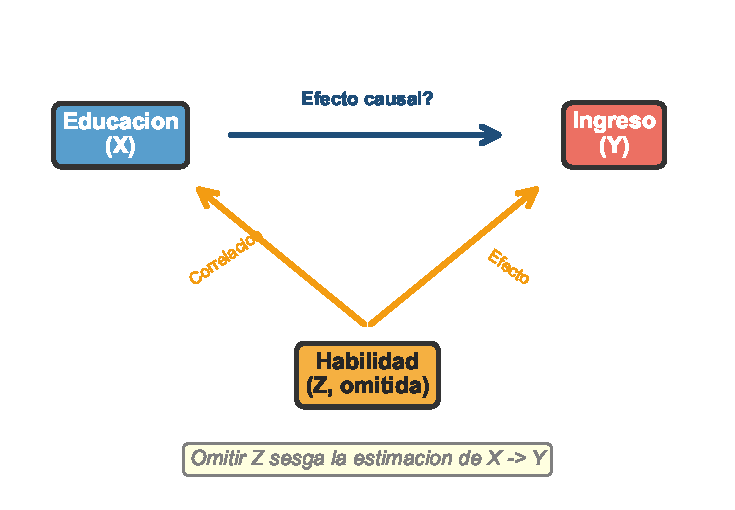
\includegraphics[height=0.7\textheight]{sesgo_variable_omitida.pdf}
\end{center}

\end{frame}

% ============================================================================
% SLIDE 7: ESTRUCTURAS CAUSALES - TRES TIPOS (NUEVA)
% ============================================================================
\begin{frame}{Estructuras Causales: Tres Tipos de Variables}
\begin{center}
    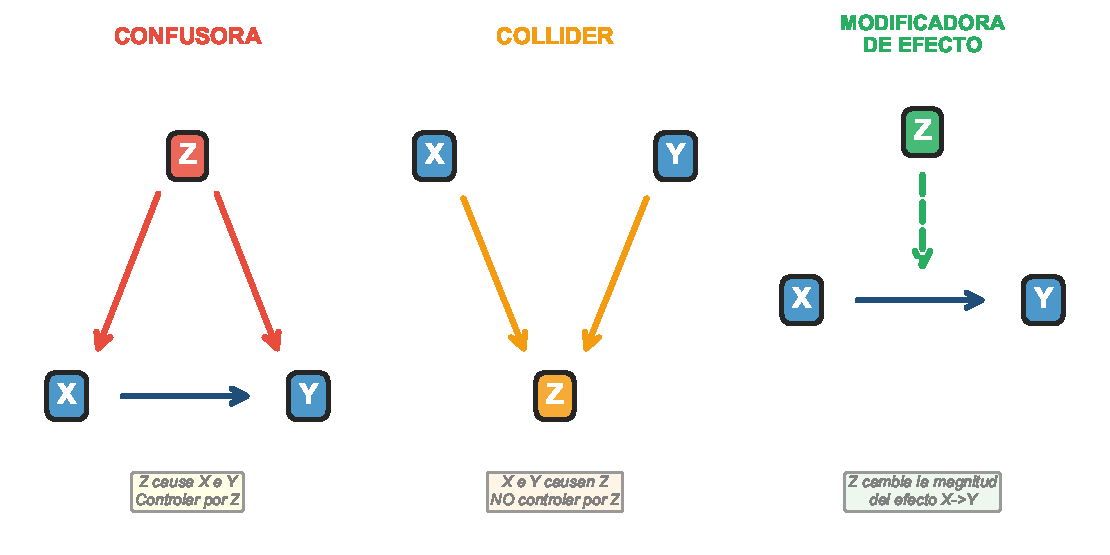
\includegraphics[height=0.75\textheight]{dag_tres_tipos.pdf}
\end{center}
\vspace{-0.2cm}
{\scriptsize Cada estructura requiere una estrategia diferente de control.}
\end{frame}

% ============================================================================
% SLIDE 8: CONFUSORA EN DETALLE (NUEVA)
% ============================================================================
\begin{frame}{Variable Confusora (Confounder)}
\small
\begin{block}{Definici\'on}
    Variable $Z$ que \textbf{causa tanto} a $X$ como a $Y$, generando asociaci\'on espuria.
\end{block}

\vspace{0.1cm}
\textbf{Estructura causal:} $X \leftarrow Z \rightarrow Y$

\vspace{0.1cm}
\textbf{C\'omo identificarla:}
\begin{itemize}
    \setlength{\itemsep}{1pt}
    \item $Z$ est\'a asociada con $X$ (exposici\'on)
    \item $Z$ afecta a $Y$ (resultado), independientemente de $X$
    \item $Z$ \textbf{no es} consecuencia de $X$ (no est\'a en el camino causal)
\end{itemize}

\vspace{0.1cm}
\textbf{Acci\'on:} \highlight{Controlar por $Z$} (incluirla en el modelo)

\vspace{0.1cm}
\begin{exampleblock}{Ejemplo}
    \scriptsize
    Efecto de educaci\'on ($X$) en ingreso ($Y$), con nivel socioecon\'omico familiar ($Z$) como confusora: familias ricas dan m\'as educaci\'on \textit{y} m\'as oportunidades laborales.
\end{exampleblock}
\end{frame}

% ============================================================================
% SLIDE 9: COLLIDER EN DETALLE (NUEVA)
% ============================================================================
\begin{frame}{Variable Collider (Colisionador)}
\small
\begin{block}{Definici\'on}
    Variable $Z$ \textbf{causada por} $X$ \textit{y} por $Y$. Controlar por ella \textbf{introduce sesgo}.
\end{block}

\vspace{0.1cm}
\textbf{Estructura causal:} $X \rightarrow Z \leftarrow Y$

\vspace{0.1cm}
\textbf{C\'omo identificarla:}
\begin{itemize}
    \setlength{\itemsep}{1pt}
    \item $Z$ es \textbf{consecuencia} de $X$ y de $Y$ (o de sus causas)
    \item $X$ e $Y$ no est\'an conectados excepto a trav\'es de $Z$
    \item Condicionar en $Z$ \textit{abre} un camino espurio entre $X$ e $Y$
\end{itemize}

\vspace{0.1cm}
\textbf{Acci\'on:} \highlight{NO controlar por $Z$}

\vspace{0.1cm}
\begin{exampleblock}{Ejemplo}
    \scriptsize
    Talento ($X$) y belleza ($Y$) son independientes, pero ambos causan fama ($Z$). Si analizamos \textit{solo famosos}, aparece correlaci\'on negativa espuria (``paradoja de Berkson'').
\end{exampleblock}
\end{frame}

% ============================================================================
% SLIDE 10: MODIFICADORA DE EFECTO (NUEVA)
% ============================================================================
\begin{frame}{Modificadora de Efecto (Effect Modifier)}
\small
\begin{block}{Definici\'on}
    Variable $Z$ que \textbf{cambia la magnitud o direcci\'on} del efecto de $X$ sobre $Y$.
\end{block}

\vspace{0.1cm}
\textbf{Estructura:} $Z$ modifica la relaci\'on $X \rightarrow Y$ (no confunde)

\vspace{0.1cm}
\textbf{C\'omo identificarla:}
\begin{itemize}
    \setlength{\itemsep}{1pt}
    \item El efecto de $X$ en $Y$ cambia seg\'un el valor de $Z$
    \item Se detecta con un \textbf{t\'ermino de interacci\'on} ($X \times Z$) significativo
    \item Estratificar por $Z$ muestra pendientes diferentes
\end{itemize}

\vspace{0.1cm}
\textbf{Acci\'on:} \highlight{Incluir interacci\'on $X \times Z$} en el modelo

\vspace{0.1cm}
\begin{exampleblock}{Ejemplo}
    \scriptsize
    El retorno a la educaci\'on ($X$) en salario ($Y$) difiere por g\'enero ($Z$): incluir $\text{Educ} \times \text{Mujer}$ para capturar esta heterogeneidad.
\end{exampleblock}
\end{frame}

% ============================================================================
% SLIDE 11: RESUMEN COMPARATIVO (NUEVA)
% ============================================================================
\begin{frame}{Resumen: ?`Controlar o No Controlar?}
\small
\begin{center}
\begin{tabular}{l|c|c|c}
\toprule
& \textbf{Confusora} & \textbf{Collider} & \textbf{Modificadora} \\
\midrule
\textbf{DAG} & $X \leftarrow Z \rightarrow Y$ & $X \rightarrow Z \leftarrow Y$ & $Z$ modifica $X \rightarrow Y$ \\
\midrule
\textbf{Si NO controlas} & Sesgo & Sin sesgo & Efecto promedio \\
\midrule
\textbf{Si controlas} & Sin sesgo & \textcolor{red}{Introduce sesgo} & Efectos por grupo \\
\midrule
\textbf{Acci\'on correcta} & \textcolor{green!60!black}{Controlar} & \textcolor{red}{No controlar} & \textcolor{green!60!black}{Interacci\'on} \\
\bottomrule
\end{tabular}
\end{center}

\vspace{0.4cm}
\textbf{Criterio pr\'actico para decidir:}
\begin{enumerate}
    \setlength{\itemsep}{2pt}
    \item Dibujar el DAG (diagrama causal) del problema
    \item Identificar si $Z$ es causa com\'un, consecuencia com\'un, o modificador
    \item Aplicar la regla correspondiente
\end{enumerate}

\vspace{0.2cm}
\footnotesize \textit{``No todo lo que correlaciona con $X$ e $Y$ debe ser un control.''}
\end{frame}

% ============================================================================
% SLIDE 12: MODELOS ANIDADOS (NUEVA)
% ============================================================================
\begin{frame}{Modelos Anidados: Detectando OVB}
\begin{center}
    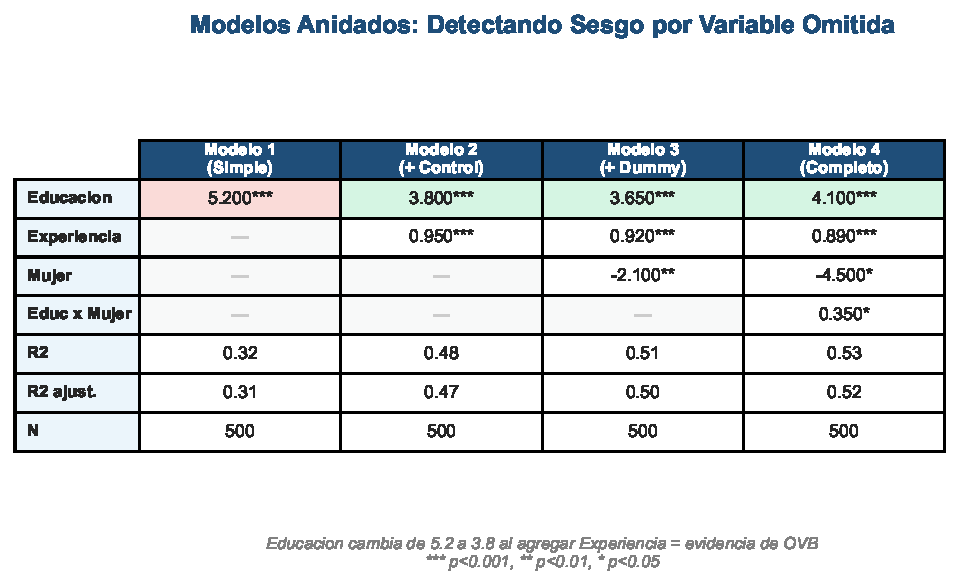
\includegraphics[height=0.78\textheight]{modelos_anidados.pdf}
\end{center}
\end{frame}

% ============================================================================
% SLIDE 13: COMO IDENTIFICAR OVB CON MODELOS ANIDADOS (NUEVA)
% ============================================================================
\begin{frame}{Identificaci\'on de Sesgos con Modelos Anidados}
\small
\begin{block}{M\'etodo}
    Estimar modelos progresivamente m\'as completos y observar c\'omo cambian los coeficientes de inter\'es.
\end{block}

\vspace{0.2cm}
\textbf{Se\~nales de OVB:}
\begin{itemize}
    \setlength{\itemsep}{3pt}
    \item El coeficiente de inter\'es \textbf{cambia sustancialmente} ($>$20\%) al agregar controles
    \item El $R^2$ aumenta considerablemente con la nueva variable
    \item La nueva variable es significativa y tiene sentido te\'orico
\end{itemize}

\vspace{0.2cm}
\textbf{Se\~nales de que NO hay OVB:}
\begin{itemize}
    \setlength{\itemsep}{3pt}
    \item El coeficiente se mantiene estable al agregar controles
    \item Los controles son significativos pero no alteran el efecto principal
\end{itemize}

\vspace{0.2cm}
\textbf{Herramienta formal: Test de Hausman}
\[
H = (\hat{\beta}_{\text{restringido}} - \hat{\beta}_{\text{completo}})^T [\text{Var}(\hat{\beta}_r) - \text{Var}(\hat{\beta}_c)]^{-1} (\hat{\beta}_r - \hat{\beta}_c) \sim \chi^2_q
\]
\end{frame}

% ============================================================================
% SLIDE 14: IMPLEMENTACION MODELOS ANIDADOS EN R (NUEVA)
% ============================================================================
\begin{frame}[fragile]{Modelos Anidados en R}
\tiny
\begin{lstlisting}
# Modelo 1: Solo variable de interes
m1 <- lm(ingreso ~ educacion, data = datos)

# Modelo 2: Agregar control (experiencia)
m2 <- lm(ingreso ~ educacion + experiencia, data = datos)

# Modelo 3: Agregar dummy (genero)
m3 <- lm(ingreso ~ educacion + experiencia + mujer, data = datos)

# Modelo 4: Agregar interaccion
m4 <- lm(ingreso ~ educacion * mujer + experiencia, data = datos)

# Comparar coeficientes lado a lado
library(stargazer)
stargazer(m1, m2, m3, m4, type = "text",
          column.labels = c("Simple","+ Control","+ Dummy","Completo"))

# Test F para comparar modelos anidados
anova(m1, m2)  # Test: es experiencia significativa?
anova(m3, m4)  # Test: es la interaccion significativa?
\end{lstlisting}
\end{frame}

% ============================================================================
% SLIDE 15: VARIABLES DE CONTROL
% ============================================================================
\begin{frame}{Variables de Control: Cu\'ando y Cu\'ales Incluir}

\small
\textbf{?`Cu\'ando incluir una variable como control?}
\begin{itemize}
    \setlength{\itemsep}{2pt}
    \item Es una \textbf{confusora}: afecta a $Y$ y est\'a correlacionada con $X$
    \item NO es un \textbf{collider}: no es consecuencia de $X$ e $Y$
    \item NO es un \textbf{mediador}: no est\'a en el camino causal $X \rightarrow Z \rightarrow Y$
\end{itemize}

\vspace{0.3cm}

\textbf{?`Cu\'ales NO incluir?}
\begin{itemize}
    \setlength{\itemsep}{2pt}
    \item Colliders: introducen sesgo (Berkson)
    \item Mediadores: absorben parte del efecto causal
    \item Variables post-tratamiento (consecuencias de $X$)
\end{itemize}

\vspace{0.3cm}

\textbf{Criterio pr\'actico:}
\begin{itemize}
    \setlength{\itemsep}{2pt}
    \item Dibujar el DAG antes de estimar
    \item Incluir variables demogr\'aficas cl\'asicas (edad, g\'enero, educaci\'on)
    \item Reportar resultados con y sin controles (modelos anidados)
\end{itemize}

\end{frame}

% ============================================================================
% SLIDE 16: DUMMY VARIABLES
% ============================================================================
\begin{frame}{Variables Categ\'oricas: Dummy Variables}

\textbf{Problema:} C\'omo incluir variables cualitativas (g\'enero, regi\'on, estado)

\vspace{0.3cm}

\textbf{Soluci\'on:} Convertir en variables binarias (0/1)

\vspace{0.2cm}

\small
\textbf{Ejemplo:} G\'enero
\[
\text{Mujer} = \begin{cases} 1 & \text{si es mujer} \\ 0 & \text{si es hombre (categor\'ia de referencia)} \end{cases}
\]

\vspace{0.2cm}

\textbf{Modelo:}
\[
\text{Salario} = \beta_0 + \beta_1 \text{Mujer} + \beta_2 \text{Educaci\'on} + \varepsilon
\]

\vspace{0.2cm}

\small
\textbf{Interpretaci\'on:}
\begin{itemize}
    \setlength{\itemsep}{2pt}
    \item $\beta_0$: salario promedio para hombres (categor\'ia de referencia)
    \item $\beta_1$: diferencia promedio de salario entre mujeres y hombres
    \item \textbf{Regla:} Para $C$ categor\'ias, crear $C-1$ variables dummy
\end{itemize}

\end{frame}

% ============================================================================
% SLIDE 17: DUMMY VISUAL
% ============================================================================
\begin{frame}{Variables Dummy: Ejemplo Visual}
\begin{center}
    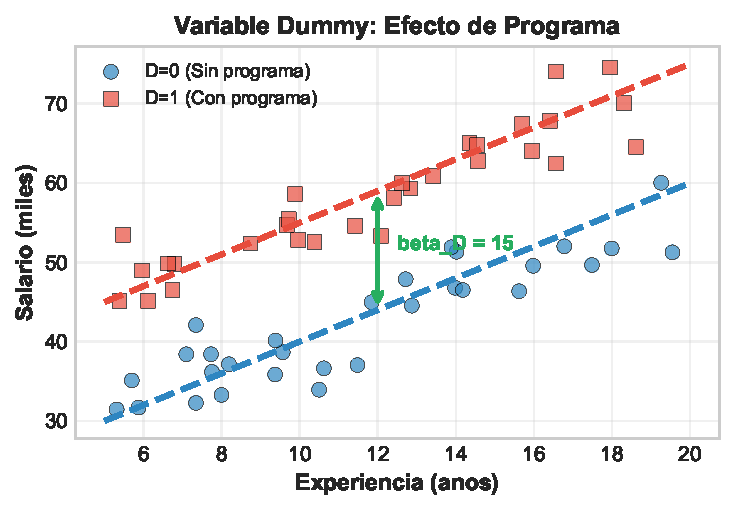
\includegraphics[height=0.78\textheight]{variables_dummy.pdf}
\end{center}
\end{frame}

% ============================================================================
% SLIDE 18: TERMINOS DE INTERACCION
% ============================================================================
\begin{frame}{T\'erminos de Interacci\'on}

\small
\textbf{Motivaci\'on:} Efecto heterog\'eneo --- El retorno a la educaci\'on ?`difiere por g\'enero?

\vspace{0.2cm}
\textbf{Modelo:}
\[
\text{Salario} = \beta_0 + \beta_1 \text{Educ} + \beta_2 \text{Mujer} + \beta_3 (\text{Educ} \times \text{Mujer}) + \varepsilon
\]

\vspace{0.2cm}
\textbf{Interpretaci\'on:}
\begin{itemize}
    \setlength{\itemsep}{3pt}
    \item $\beta_1$: retorno a educaci\'on para hombres (grupo base)
    \item $\beta_2$: diferencia de intercepto (mujeres vs hombres, cuando Educ=0)
    \item $\beta_3$: \highlight{diferencia en retorno} de educaci\'on (mujeres vs hombres)
    \item Retorno para mujeres: $\beta_1 + \beta_3$
\end{itemize}

\vspace{0.2cm}
\begin{exampleblock}{Conexi\'on con modificadora de efecto}
    \small Si $\beta_3$ es significativo, el g\'enero es una \textbf{modificadora de efecto} del retorno a la educaci\'on.
\end{exampleblock}
\end{frame}

% ============================================================================
% SLIDE 19: INTERACCION VISUAL
% ============================================================================
\begin{frame}{Interacci\'on: Ejemplo Visual}
\begin{center}
    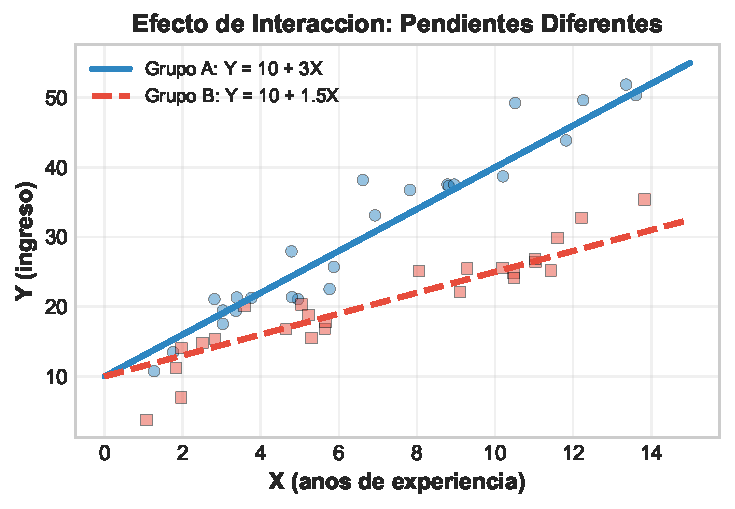
\includegraphics[height=0.78\textheight]{interaccion.pdf}
\end{center}
\end{frame}

% ============================================================================
% SLIDE 20: PRUEBA T INDIVIDUAL
% ============================================================================
\begin{frame}{Pruebas de Significancia Individual (t-test)}

\textbf{Pregunta:} ?`Es el coeficiente $\hat{\beta}_j$ estad\'isticamente diferente de cero?

\vspace{0.3cm}

\small
\textbf{Hip\'otesis nula:} $H_0: \beta_j = 0$ (la variable no afecta a $Y$)

\textbf{Estad\'istico de prueba:}
\[
t = \frac{\hat{\beta}_j}{\text{EE}(\hat{\beta}_j)} \sim t_{n-k-1}
\]

\vspace{0.2cm}

\textbf{Decisi\'on (al nivel $\alpha = 0.05$):}
\begin{itemize}
    \setlength{\itemsep}{2pt}
    \item Si $|t| > 1.96$ (aprox): rechazamos $H_0$ --- variable significativa
    \item Notaci\'on en tablas: \texttt{***} $p < 0.001$, \texttt{**} $p < 0.01$, \texttt{*} $p < 0.05$
\end{itemize}

\vspace{0.2cm}

\textbf{Intervalo de confianza al 95\%:}
\[
\hat{\beta}_j \pm t_{\alpha/2} \cdot \text{EE}(\hat{\beta}_j)
\]

\end{frame}

% ============================================================================
% SLIDE 21: PRUEBA F CONJUNTA
% ============================================================================
\begin{frame}{Pruebas de Significancia Conjunta (F-test)}
\small
\textbf{Pregunta:} ?`Son \textbf{conjuntamente} significativas un grupo de coeficientes?

\vspace{0.2cm}

\textbf{Hip\'otesis nula:} $H_0: \beta_1 = \beta_2 = \cdots = \beta_q = 0$

\vspace{0.2cm}

\textbf{Estad\'istico F:}
\[
F = \frac{(R^2_u - R^2_r) / q}{(1 - R^2_u) / (n - k - 1)} \sim F_{q, n-k-1}
\]

\vspace{0.2cm}

\begin{itemize}
    \setlength{\itemsep}{2pt}
    \item $R^2_u$: modelo no restringido (completo)
    \item $R^2_r$: modelo restringido (sin las variables testeadas)
    \item $q$: n\'umero de restricciones
\end{itemize}

\vspace{0.2cm}

\textbf{Aplicaci\'on clave:} Comparar modelos anidados con \texttt{anova(m1, m2)} en R.
\end{frame}

% ============================================================================
% SLIDE 22: MULTICOLINEALIDAD
% ============================================================================
\begin{frame}{Multicolinealidad}
\small
\textbf{Definici\'on:} Correlaci\'on alta entre regresores

\vspace{0.2cm}

\textbf{?`Por qu\'e es un problema?}
\begin{itemize}
    \setlength{\itemsep}{2pt}
    \item Aumenta varianza de estimadores: $\text{Var}(\hat{\beta}_j) = \frac{\sigma^2}{(1-R_j^2) \sum (X_j - \bar{X}_j)^2}$
    \item Intervalos de confianza m\'as amplios
    \item Dificultad para separar efectos individuales
\end{itemize}

\vspace{0.2cm}

\textbf{Detecci\'on: Factor de Inflaci\'on de Varianza (VIF)}
\[
\text{VIF}_j = \frac{1}{1 - R_j^2}
\]

\begin{itemize}
    \setlength{\itemsep}{2pt}
    \item VIF = 1: sin colinealidad
    \item VIF $<$ 5: aceptable
    \item VIF $>$ 10: problem\'atico
\end{itemize}

\vspace{0.1cm}
\footnotesize
\textcolor{uddlight}{\textbf{Nota:} Multicolinealidad NO causa sesgo, solo reduce precisi\'on.}
\end{frame}

% ============================================================================
% SLIDE 23: VIF VISUAL
% ============================================================================
\begin{frame}{Diagn\'ostico de Multicolinealidad: VIF}
\begin{center}
    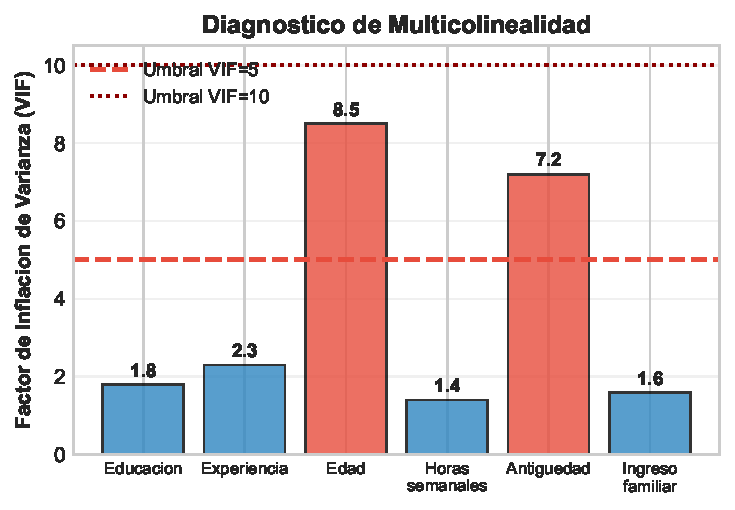
\includegraphics[height=0.78\textheight]{vif_multicolinealidad.pdf}
\end{center}
\end{frame}

% ============================================================================
% SLIDE 24: IMPLEMENTACION EN R
% ============================================================================
\begin{frame}[fragile]{Implementaci\'on en R: Estimaci\'on y Diagn\'osticos}
\tiny
\begin{lstlisting}
# Estimar modelos
datos <- read.csv("datos.csv")
m1 <- lm(Y ~ X1, data = datos)
m2 <- lm(Y ~ X1 + X2 + X3, data = datos)
m3 <- lm(Y ~ X1 * factor(genero) + X2, data = datos)

# Resumen
summary(m2)

# VIF
library(car)
vif(m2)

# Comparar modelos anidados
anova(m1, m2)

# Tabla profesional
library(stargazer)
stargazer(m1, m2, m3, type = "text")
\end{lstlisting}
\end{frame}

% ============================================================================
% SLIDE 25: EJERCICIO PRACTICO
% ============================================================================
\begin{frame}{Ejercicio Pr\'actico}
\small
\textbf{Dataset \texttt{mtcars}:} Modelar consumo de combustible (\texttt{mpg})

\vspace{0.3cm}
\textbf{Tareas:}
\begin{enumerate}
    \setlength{\itemsep}{4pt}
    \item Estimar modelos anidados:
    \begin{itemize}
        \small
        \item M1: \texttt{mpg $\sim$ wt}
        \item M2: \texttt{mpg $\sim$ wt + hp}
        \item M3: \texttt{mpg $\sim$ wt + hp + factor(cyl)}
        \item M4: \texttt{mpg $\sim$ wt * am + hp + factor(cyl)}
    \end{itemize}
    \item Comparar coeficientes: ?`hay evidencia de OVB en M1?
    \item Calcular VIF en M3
    \item Si la interacci\'on en M4 es significativa, ?`qu\'e tipo de variable es \texttt{am}?
\end{enumerate}
\end{frame}

% ============================================================================
% SLIDE 26: RESUMEN
% ============================================================================
\begin{frame}{Resumen}
\small
\begin{itemize}
    \setlength{\itemsep}{4pt}
    \item \textbf{OVB:} Omitir confusoras sesga coeficientes; usar modelos anidados para detectar

    \item \textbf{Tres estructuras causales:}
    \begin{itemize}
        \small
        \item Confusora ($X \leftarrow Z \rightarrow Y$): controlar
        \item Collider ($X \rightarrow Z \leftarrow Y$): \textbf{no} controlar
        \item Modificadora: incluir interacci\'on
    \end{itemize}

    \item \textbf{Modelos anidados:} Si $\hat{\beta}$ cambia $>$20\% al agregar control $\rightarrow$ evidencia de OVB

    \item \textbf{Variables dummy} para categ\'oricas ($C-1$ dummies); \textbf{interacciones} para efectos heterog\'eneos

    \item \textbf{Pruebas t} (individual) y \textbf{F} (conjunta/anidados); \textbf{VIF} para multicolinealidad
\end{itemize}

\vspace{0.3cm}
\textbf{Pr\'oxima sesi\'on:} Pr\'actica integradora en R

\vspace{0.3cm}
\centering
\Large \highlight{?`Preguntas?}
\end{frame}

\end{document}
